\documentclass[11pt]{article}

% ====================================================
% PACKAGES
% ====================================================
\usepackage[margin=1in, headheight=13.6pt]{geometry}
\usepackage[T1]{fontenc}
\usepackage{lmodern}
\usepackage{microtype}
\usepackage{setspace}
\usepackage{tcolorbox}
\usepackage{amsmath, amssymb, mathtools}
\usepackage{siunitx}

\usepackage{graphicx}
\usepackage{float}
\usepackage{subcaption}

\usepackage{enumitem}
\usepackage{booktabs}
\usepackage{longtable}
\usepackage{array}
\usepackage{multirow}

\usepackage{xcolor}
\usepackage{hyperref}

\usepackage{fancyhdr}
\usepackage{lastpage}

\usepackage{listings}
\usepackage{indentfirst}
\usepackage[justification=centering]{caption}

% Python source style for \CodeListing
\lstdefinestyle{pystyle}{
    language=Python,
    basicstyle=\ttfamily\footnotesize,
    keywordstyle=\color{blue!60!black}\bfseries,
    stringstyle=\color{orange!70!black},
    commentstyle=\color{gray!60!black}\itshape,
    numbers=left,
    numberstyle=\tiny\color{gray!70},
    numbersep=8pt,
    breaklines=true,
    showstringspaces=false,
    frame=single,
    rulecolor=\color{gray!40},
    tabsize=4,
    columns=fullflexible,
    captionpos=b,
    literate={°}{{\textdegree}}1,
}
\lstset{style=pystyle}

\pagestyle{fancy}
\fancyhf{}
\lhead{\Assignment\ |\ \course}
\rhead{\Name\ |\ \today}
\cfoot{Page \thepage\ of~\pageref{LastPage}}

\hypersetup{
    colorlinks,
    linkcolor={red!50!black},
    citecolor={blue!50!black},
    urlcolor={blue!80!black}
}

\newcommand{\Name}{Arael Anaya}
\newcommand{\Assignment}{Homework 2}
\newcommand{\course}{Advanced Dynamics}

% Boxed final-answer environment
\newtcolorbox{result}{
    colback=blue!3!white,
    colframe=blue!40!black,
    boxrule=0.6pt,
    arc=2pt,
    left=6pt, right=6pt, top=4pt, bottom=4pt
}

% Code listing: sources the .py file directly.
\newcommand{\CodeListing}[3]{%
\IfFileExists{#1}%
    {\lstinputlisting[style=pystyle,caption={#2},label={#3}]{#1}}%
    {\begin{quote}\itshape Source file \texttt{#1} not found yet --- this
        listing will populate automatically once the file is written.\end{quote}}}

\begin{document}

% ====================================================
% PROBLEM 1
% ====================================================
\section*{Problem 1}

\begin{figure}[H]
    \centering
    
\includegraphics[width=0.8\linewidth]{Figures/Problem Set/Problem 1.png}
\end{figure}

\subsection*{Setup}

Let $r$ be the crank length $MA$, $h$ the height of $M$ above $O$, and $H$ the height of the slot above $O$. With $q_1=x$, $q_2=\theta$,
\[
    \vec r_{OA} = r\cos\theta\,\hat n_1 + \big(h-r\sin\theta\big)\hat n_2,
    \qquad
    \vec r_{OB} = x\,\hat n_1 + H\,\hat n_2
\]

\subsection*{Part (a): Constraint Equation}

Since $O$, $A$, $B$ are collinear, $\vec r_{OA}\times\vec r_{OB}=\vec 0$:
\[
    r\cos\theta\cdot H - \big(h-r\sin\theta\big)x = 0
\]
\begin{result}
\[
    \phi_1:\quad x\big(h-r\sin\theta\big) - Hr\cos\theta = 0
\]
\end{result}

\subsection*{Part (b): Coefficients $a_{11}$, $a_{12}$}

\[
    \dot\phi_1 = \frac{\partial\phi_1}{\partial x}\dot x + \frac{\partial\phi_1}{\partial\theta}\dot\theta
    = a_{11}\dot x + a_{12}\dot\theta
\]
\[
    \frac{\partial\phi_1}{\partial x} = h-r\sin\theta,
    \qquad
    \frac{\partial\phi_1}{\partial\theta} = r\big(H\sin\theta - x\cos\theta\big)
\]
\begin{result}
\[
    a_{11} = h - r\sin\theta,
    \qquad
    a_{12} = r\big(H\sin\theta - x\cos\theta\big)
\]
\end{result}

\subsection*{Part (c): Solving for $\dot x$}

\[
    \dot\phi_1 = 0
    \;\Rightarrow\;
    \dot x = -\frac{a_{12}}{a_{11}}\dot\theta
\]
Substituting $x = \dfrac{Hr\cos\theta}{h-r\sin\theta}$ from part (a) into $a_{12}$:
\[
    a_{12} = r\big(H\sin\theta - x\cos\theta\big)
    = \frac{rH\big(h\sin\theta - r\big)}{h-r\sin\theta}
\]
so that
\[
    \dot x = -\frac{a_{12}}{a_{11}}\dot\theta = -\frac{rH\big(h\sin\theta-r\big)}{(h-r\sin\theta)^2}\dot\theta
\]
\begin{result}
\[
    \dot x = \frac{Hr\big(r-h\sin\theta\big)}{\big(h-r\sin\theta\big)^{2}}\,\dot\theta
\]
\end{result}

\subsection*{Part (d): Numerical Results}

$\dot\theta = 5\ \text{rad/s}$ (constant), $r=1\ \text{m}$, $h=10\ \text{m}$, $H=20\ \text{m}$, $\theta\in[0,2\pi]$.

\begin{figure}[H]
    \centering
    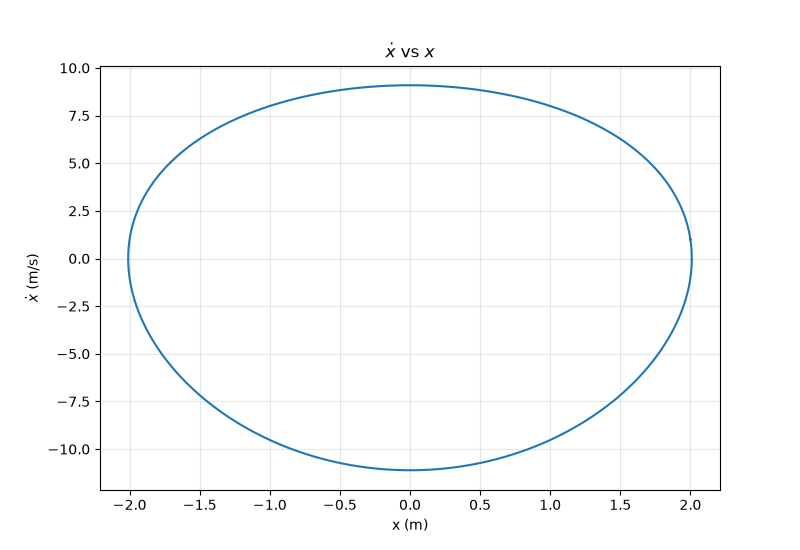
\includegraphics[width=0.8\linewidth]{Figures/Graphs/X vs X_dot.png}
    \caption{$\dot x$ vs.\ $x$ over one full crank revolution.}
    \label{fig:p1_x_xdot}
\end{figure}

\begin{figure}[H]
    \centering
    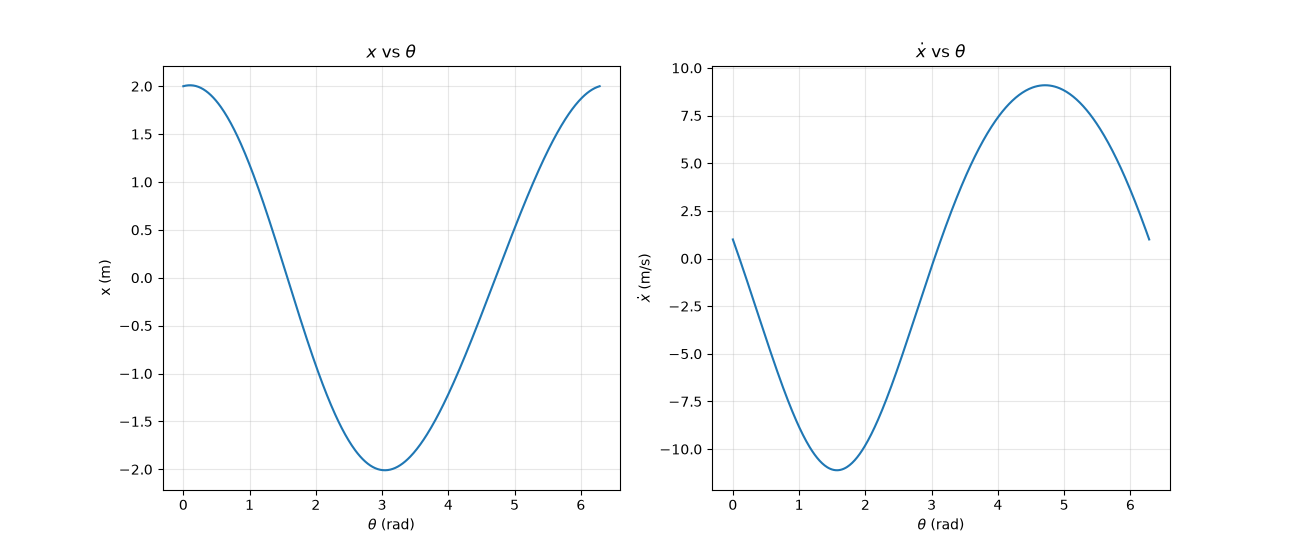
\includegraphics[width=0.8\linewidth]{Figures/Graphs/X and X_dot vs Theta.png}
    \caption{$x$ and $\dot x$ vs.\ $\theta$. Near $\theta=\pi/2$, $\dot x$ reaches its most negative value (brief, fast return); near $\theta=3\pi/2$, $\dot x$ reaches a smaller-magnitude positive peak spread over more of the cycle (slow stroke) --- the quick-return behavior of the Whitworth mechanism.}
    \label{fig:p1_theta}
\end{figure}

% ====================================================
% PROBLEM 2
% ====================================================
\newpage
\section*{Problem 2}

\begin{figure}[H]
    \centering
    
\includegraphics[width=0.8\linewidth]{Figures/Problem Set/Problem 2.png}
\end{figure}

\subsection*{Positions}

With $\hat e_z$ pointing down, $\hat e_x$ horizontal, and $\theta$ measured from $\hat e_z$ so that $\hat e_r = \sin\theta\,\hat e_x+\cos\theta\,\hat e_z$,
\begin{result}
\[
    \vec r_1 = 2\ell\cos\theta\,\hat e_z,
    \qquad
    \vec r_2 = \ell\,\hat e_r = \ell\sin\theta\,\hat e_x + \ell\cos\theta\,\hat e_z
\]
\end{result}

\subsection*{Velocities and Inertial Accelerations}

\[
    \dot{\vec r}_1 = -2\ell\sin\theta\,\dot\theta\,\hat e_z,
    \qquad
    \dot{\vec r}_2 = \ell\cos\theta\,\dot\theta\,\hat e_x - \ell\sin\theta\,\dot\theta\,\hat e_z
\]
\begin{result}
\begin{align*}
    \ddot{\vec r}_1 &= -2\ell\big(\dot\theta^{2}\cos\theta+\ddot\theta\sin\theta\big)\hat e_z\\
    \ddot{\vec r}_2 &= \ell\big(\ddot\theta\cos\theta-\dot\theta^{2}\sin\theta\big)\hat e_x
        - \ell\big(\ddot\theta\sin\theta+\dot\theta^{2}\cos\theta\big)\hat e_z
\end{align*}
\end{result}

\subsection*{Virtual Displacements}

\[
    \delta\vec r_i = \frac{\partial\vec r_i}{\partial\theta}\,\delta\theta
\]
\begin{result}
\[
    \delta\vec r_1 = -2\ell\sin\theta\,\delta\theta\,\hat e_z,
    \qquad
    \delta\vec r_2 = \ell\cos\theta\,\delta\theta\,\hat e_x - \ell\sin\theta\,\delta\theta\,\hat e_z
\]
\end{result}

\subsection*{Applied Forces}

\begin{result}
\[
    \vec F_{A1} = m_1 g\,\hat e_z,
    \qquad
    \vec F_{A2} = m_2 g\,\hat e_z
\]
\end{result}

\subsection*{Equation of Motion (D'Alembert's Principle)}

\[
    \sum_{i=1}^{2}\big(\vec F_{Ai}-m_i\ddot{\vec r}_i\big)\cdot\gamma_{i1} = 0,
    \qquad
    \gamma_{i1} = \frac{\partial\dot{\vec r}_i}{\partial\dot\theta} = \frac{\partial\vec r_i}{\partial\theta}
\]
\[
    \gamma_{11} = -2\ell\sin\theta\,\hat e_z,
    \qquad
    \gamma_{21} = \ell\cos\theta\,\hat e_x - \ell\sin\theta\,\hat e_z
\]

Projecting each particle's contribution onto $\gamma_{i1}$:
\begin{align*}
    \big(\vec F_{A1}-m_1\ddot{\vec r}_1\big)\cdot\gamma_{11}
        &= -2\ell m_1 g\sin\theta - 4\ell^{2}m_1\sin\theta\big(\dot\theta^{2}\cos\theta+\ddot\theta\sin\theta\big)\\
    \big(\vec F_{A2}-m_2\ddot{\vec r}_2\big)\cdot\gamma_{21}
        &= -\ell m_2 g\sin\theta - \ell^{2}m_2\ddot\theta
\end{align*}

Adding, dividing by $-\ell$, and collecting terms in $\ddot\theta$, $\dot\theta^2$, and $\sin\theta$:
\begin{result}
\[
    \big(m_2+4m_1\sin^{2}\theta\big)\ell\ddot\theta
    + \big(4m_1\ell\sin\theta\cos\theta\big)\dot\theta^{2}
    + \big(2m_1+m_2\big)g\sin\theta = 0
\]
\end{result}

\subsection*{Natural Frequency}

For small $\theta$: $\sin\theta\approx\theta$, $\cos\theta\approx1$, and $\sin^2\theta$, $\dot\theta^2\theta$ terms are negligible, so
\[
    m_2\ell\ddot\theta + \big(2m_1+m_2\big)g\theta = 0
    \;\Rightarrow\;
    \omega_n^{2} = \frac{(2m_1+m_2)g}{m_2\ell}
\]
\begin{result}
\[
    f = \frac{1}{2\pi}\sqrt{\frac{(2m_1+m_2)g}{m_2\ell}}
\]
\end{result}

% ====================================================
% PROBLEM 3
% ====================================================
\newpage
\section*{Problem 3}

\begin{figure}[H]
    \centering
    
\includegraphics[width=0.8\linewidth]{Figures/Problem Set/Problem 3.png}
\end{figure}

\subsection*{Positions}

With generalized coordinates $x_R$ (ramp) and $x_B$ (block, measured down the ramp),
\begin{result}
\[
    \vec r_1 = x_R\,\hat n_1,
    \qquad
    \vec r_2 = \big(x_R+x_B\cos\alpha\big)\hat n_1 + \big(y_0-x_B\sin\alpha\big)\hat n_2
\]
\end{result}

\subsection*{Velocities and Accelerations}

\[
    \dot{\vec r}_1 = \dot x_R\,\hat n_1,
    \qquad
    \dot{\vec r}_2 = \big(\dot x_R+\dot x_B\cos\alpha\big)\hat n_1 - \dot x_B\sin\alpha\,\hat n_2
\]
\begin{result}
\[
    \ddot{\vec r}_1 = \ddot x_R\,\hat n_1,
    \qquad
    \ddot{\vec r}_2 = \big(\ddot x_R+\ddot x_B\cos\alpha\big)\hat n_1 - \ddot x_B\sin\alpha\,\hat n_2
\]
\end{result}

\subsection*{Virtual-Displacement Coefficients}

\[
    \gamma_{ij} = \frac{\partial\dot{\vec r}_i}{\partial\dot q_j}
\]
\begin{result}
\[
    \gamma_{11}=\hat n_1,\quad \gamma_{12}=\vec 0,
    \qquad
    \gamma_{21}=\hat n_1,\quad \gamma_{22}=\cos\alpha\,\hat n_1 - \sin\alpha\,\hat n_2
\]
\end{result}

\subsection*{Applied Forces}

\[
    \vec F_{A1} = -Mg\,\hat n_2,
    \qquad
    \vec F_{A2} = -mg\,\hat n_2
\]

\subsection*{Equations of Motion (D'Alembert's Principle)}

For $q_1=x_R$: since $\vec F_{A1},\vec F_{A2}\perp\hat n_1$, gravity drops out and
\[
    \big(-M\ddot{\vec r}_1\big)\cdot\hat n_1 + \big(-m\ddot{\vec r}_2\big)\cdot\hat n_1 = 0
\]
\begin{result}
\[
    (M+m)\ddot x_R + m\cos\alpha\,\ddot x_B = 0
\]
\end{result}

For $q_2=x_B$: only particle 2 contributes, since $\gamma_{12}=\vec 0$,
\[
    \big(\vec F_{A2}-m\ddot{\vec r}_2\big)\cdot\gamma_{22} = 0
    \;\Rightarrow\;
    mg\sin\alpha - m\big(\ddot x_R\cos\alpha+\ddot x_B\big) = 0
\]
\begin{result}
\[
    \ddot x_B + \ddot x_R\cos\alpha = g\sin\alpha
\]
\end{result}

\subsection*{Solving the System}

Eliminating $\ddot x_R$ between the two boxed equations above:
\begin{result}
\begin{align*}
    \ddot x_R &= -\frac{mg\sin\alpha\cos\alpha}{M+m\sin^{2}\alpha}\\[4pt]
    \ddot x_B &= \frac{(M+m)g\sin\alpha}{M+m\sin^{2}\alpha}
\end{align*}
\end{result}

% ====================================================
% APPENDIX
% ====================================================
\newpage
\appendix
\section*{Appendix: Code Listings}

\subsection*{Problem 1 Code}
\CodeListing{../code/Problem1.py}{Numerical evaluation of $x$ and $\dot x$ vs.\ $\theta$ for the Whitworth quick-return mechanism, and generation of Figures~\ref{fig:p1_x_xdot}--\ref{fig:p1_theta}.}{lst:p1}

\end{document}
